% !TeX root = ../CourseReport.tex
%=============================================================================
%  PART 2 --- PROJECT MANAGEMENT REPORT
%  PAGE BUDGET: 8 pages (excluding title, ToC)          Rubric weight: 20 pts
%
%  Required sections (all expected by the grading criteria):
%    - Overall Project Vision (scope, key deliverables, boundaries)
%    - Project Timeline (stand-alone Gantt chart, categories, subtasks, owners)
%    - System Architecture (structure + main components)
%    - Method (methodologies; MUST include a Prompt Engineering subsection)
%    - Team Chart (members, roles, contributions)
%    - Current Progress and Future Plans
%    - Pitch Video (~60s) -- submitted as an attachment; link it here
%=============================================================================
\chapter{Project Management Report}
\label{ch:project-management}

\section{Overall Project Vision}
% TODO: Project scope, key deliverables, and explicit boundaries (what is out of
% scope). State the problem and the target outcome.

\section{Project Timeline}
% TODO: Insert a STAND-ALONE Gantt chart (readable without the surrounding text).
% Cluster work into categories (feature/team categories); show key subtasks only
% (not every task); make crew/person responsibilities clear.
% Options: pgfgantt package, or export an image and \includegraphics it.
\begin{figure}[!ht]
    \centering
    \fbox{\rule{0pt}{55mm}\rule{130mm}{0pt}}%
    % \includegraphics[width=\textwidth]{./Ressourcen/gantt.png}
    \caption{Project timeline and milestones (Gantt chart).}
    \label{fig:pm-gantt}
\end{figure}

\section{System Architecture}
% TODO: Technical details of the system structure and main components
% (gateway, recommendation, retrieval, reasoning, ingest, indexing, user;
% Qdrant, Keycloak; web + iOS clients).
\begin{figure}[!ht]
    \centering
    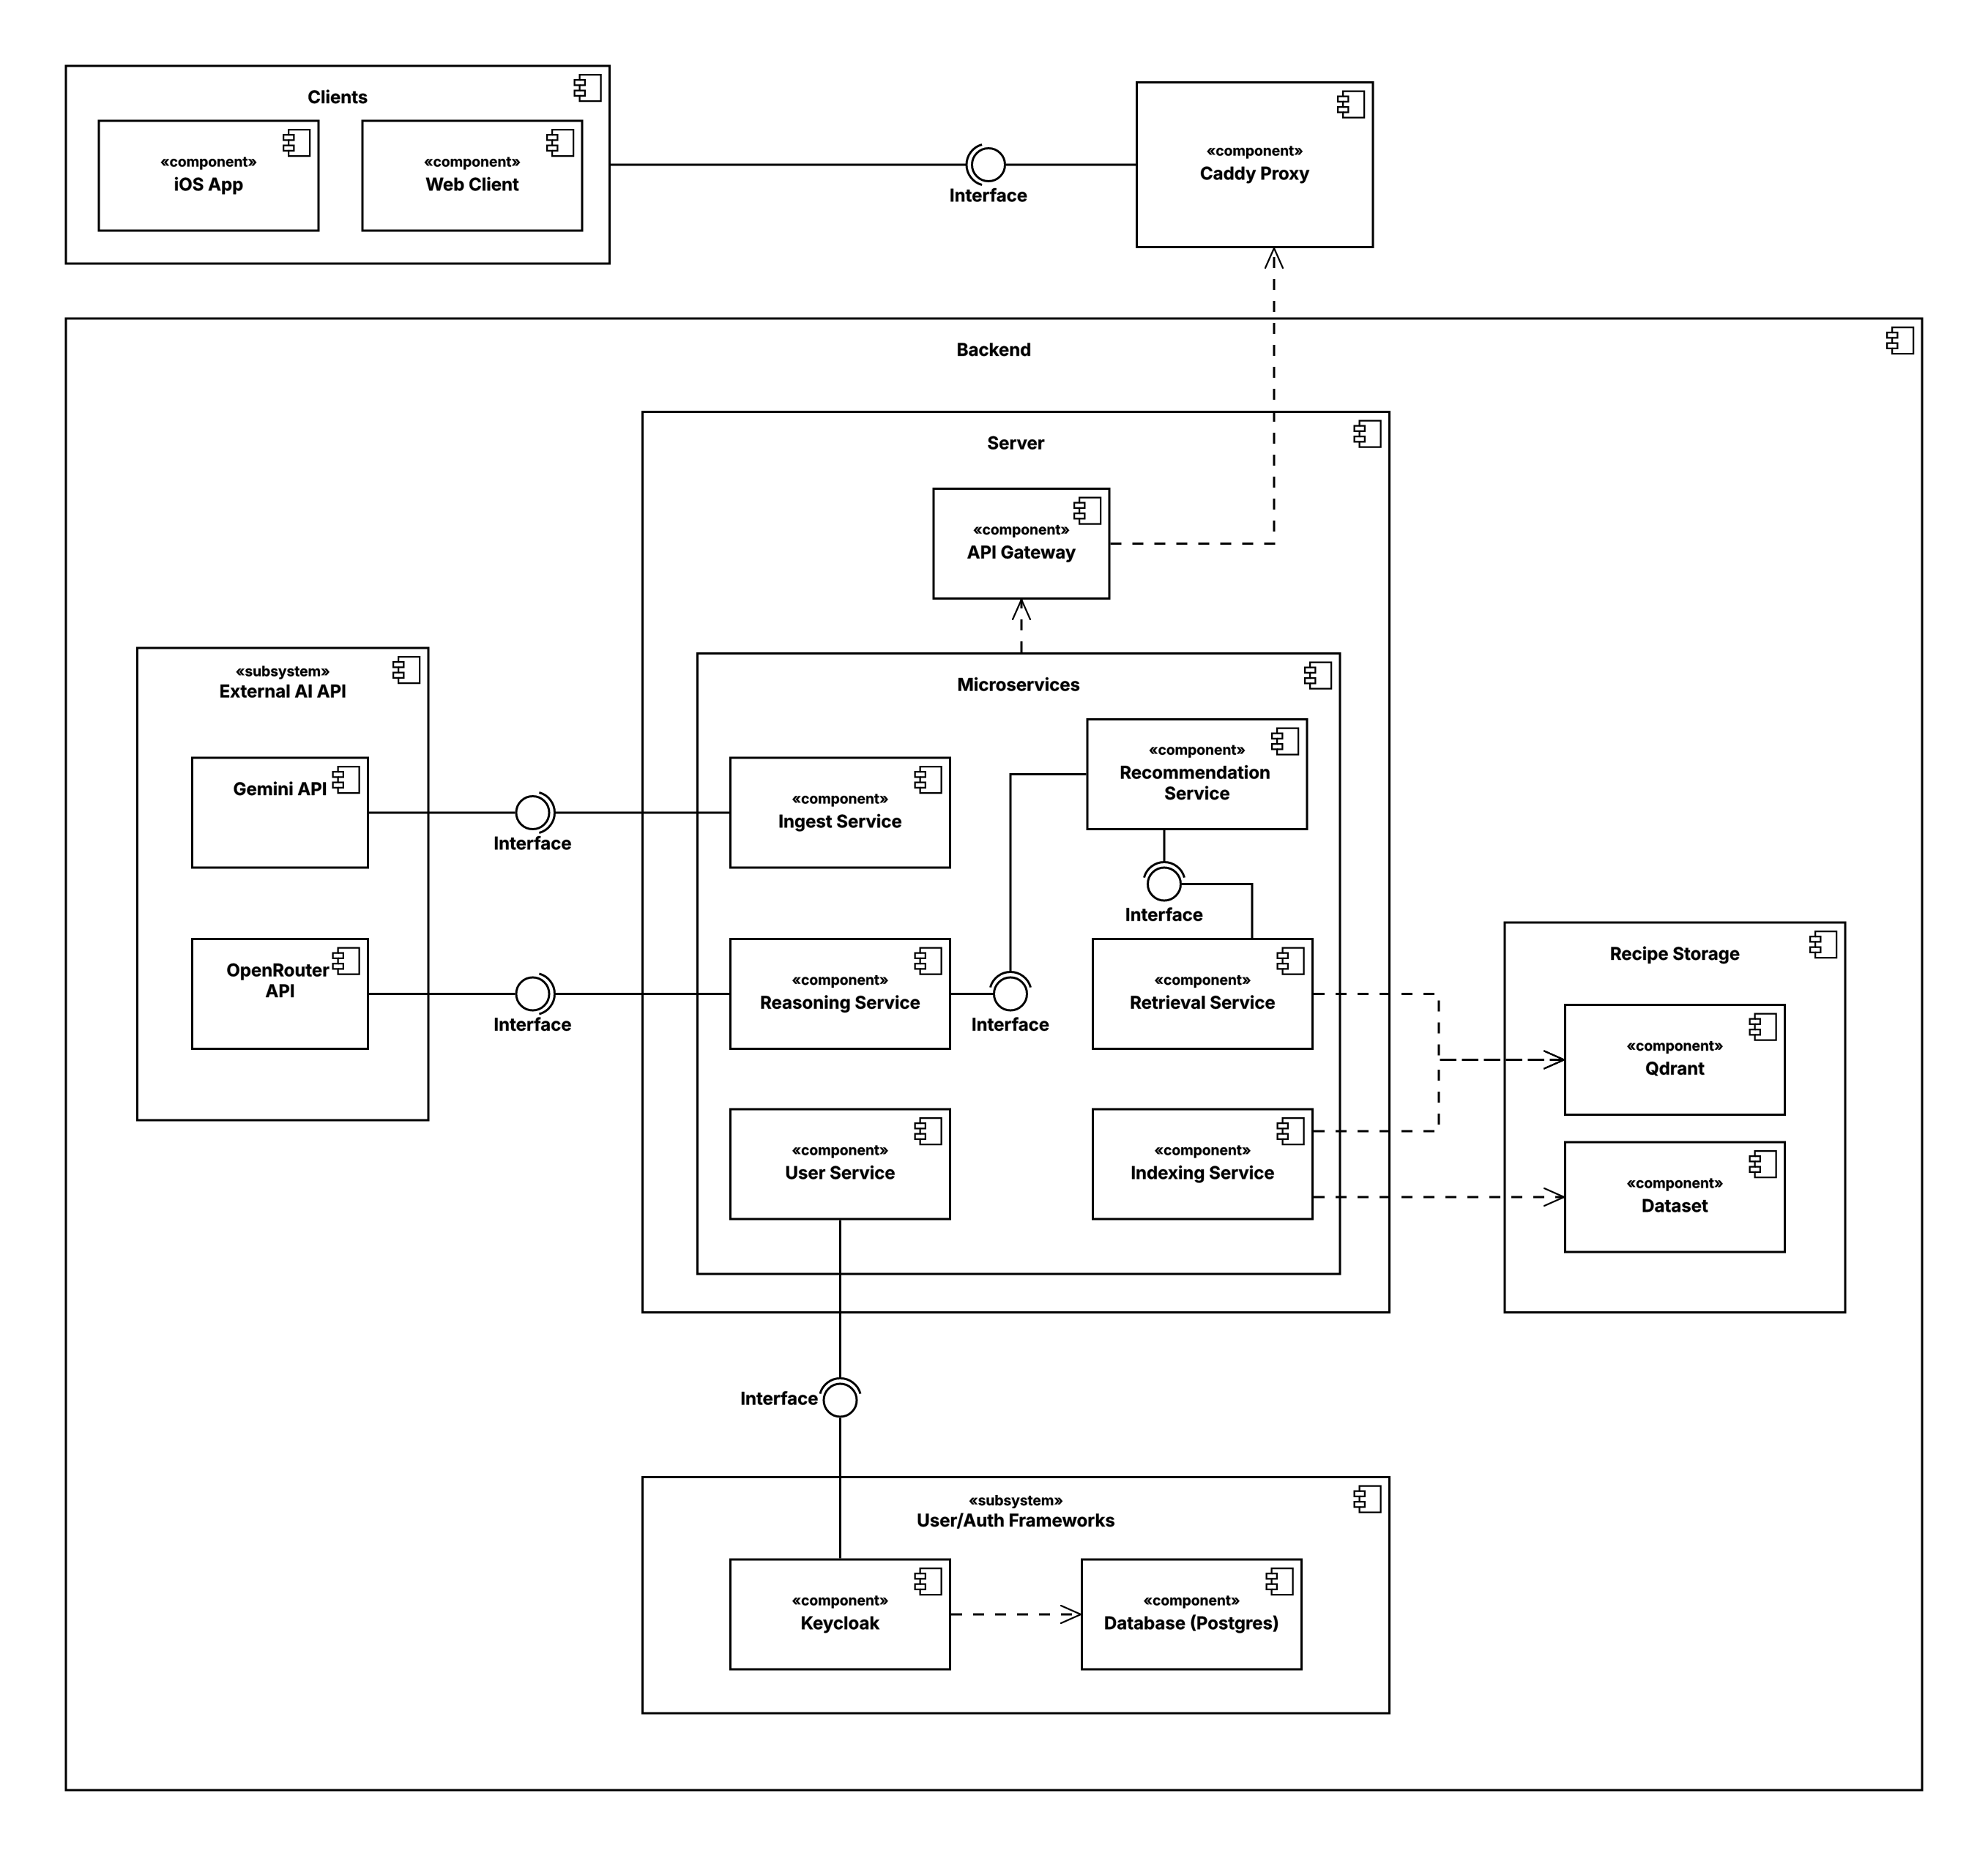
\includegraphics[width=\textwidth]{./Ressourcen/dishify_arch.png}
    \caption{Dishify system architecture and request flow.}
    \label{fig:pm-arch}
\end{figure}

\section{Method}
% TODO: Methodologies, techniques, and approaches used across the project.

\subsection{Prompt Engineering}
% TODO (REQUIRED): Prompt engineering strategies used, and how they improved the
% effectiveness of the GenAI features (reasoning explanations, recipe
% augmentation, voice/vision ingestion). Include concrete prompt patterns.

\section{Team Chart}
% TODO: Table of members, their roles, and specific contributions.
\begin{table}[!ht]
    \centering
    \caption{Team members, roles, and contributions.}
    \label{tab:pm-team}
    \begin{tabular}{@{}p{55mm}p{35mm}p{55mm}@{}}
        \toprule
        \textbf{Member} & \textbf{Role} & \textbf{Main contributions} \\
        \midrule
        Maria Chatzipavlou Arvaniti & TODO & TODO \\
        Aymen Faouel                & TODO & TODO \\
        Can Lin                     & TODO & TODO \\
        Georg Tichy                 & TODO & TODO \\
        George Trump                & TODO & TODO \\
        Chengjie Zhou               & TODO & TODO \\
        \bottomrule
    \end{tabular}
\end{table}

\section{Current Progress and Future Plans}
% TODO: Detailed status update on current progress + concrete future plans for
% project completion.

\section{Pitch Video}
% TODO: Add the link to the ~60s pitch video (also submitted as attachment).
% \url{...}
